\documentclass[12pt]{article}
\newcommand\tab[1][0.5cm]{\hspace*{#1}}
\usepackage[utf8]{inputenc}
\usepackage{listings}
\usepackage{hyperref}
\usepackage{color}
\pagenumbering{gobble}
\usepackage{changepage}
\usepackage{titletoc}
\usepackage{titlesec}
\usepackage{multicol}
\usepackage{graphicx}

\usepackage{makecell}

\definecolor{codegreen}{rgb}{0,0.6,0}
\definecolor{codegray}{rgb}{0.5,0.5,0.5}
\definecolor{codepurple}{rgb}{0.58,0,0.82}
\definecolor{backcolour}{rgb}{0.95,0.95,0.92}

\hypersetup{
	colorlinks,
	citecolor=black,
	filecolor=black,
	linkcolor=black,
	urlcolor=black
}

\lstdefinestyle{mystyle}{
	backgroundcolor=\color{backcolour},   
	commentstyle=\color{codegreen},
	keywordstyle=\color{magenta},
	numberstyle=\tiny\color{codegray},
	stringstyle=\color{codepurple},
	basicstyle=\footnotesize\ttfamily,
	breakatwhitespace=false,         
	breaklines=true,                 
	captionpos=b,                    
	keepspaces=true,                 
	numbers=left,                    
	numbersep=5pt,                  
	showspaces=false,                
	showstringspaces=false,
	showtabs=false,                  
	tabsize=2
}

\lstset{style=mystyle}

\newcommand{\titledate}[2][2.5in]{%
	\noindent%
	\begin{tabular}{@{}p{#1}@{}}
		\\ \hline \\[-.75\normalbaselineskip]
		#2
	\end{tabular} \hspace{1in}
	\begin{tabular}{@{}p{#1}@{}}
		\\ \hline \\[-.75\normalbaselineskip]
		Date
	\end{tabular}
}

\titleformat{\section}{\normalfont\Large\bfseries}{}{0pt}{}

% for forcing tables to fit
\usepackage{changepage}

\begin{document}
	

\begin{titlepage}
	
\author{Eric Pereira}
\date{Septemer 17\textsuperscript{th}, 2019}
\title{CSE4501 -- Vulnerability Research:\\Lab 2}

\maketitle

\end{titlepage}

\titlecontents{section}[0em]
{\vskip 0.5ex}%
{\scshape}% numbered sections formattin
{\itshape}% unnumbered sections formatting
{}%

\tableofcontents

\newpage \pagenumbering{arabic}

Use the necessary tools to perform analysis of the compiled source code generated. Since we
are working in 32-bit use “-m32” for your gcc compilation options. For compilation I would
suggest using compiler option ``\texttt{-fno-stack-protector}". Please submit write-ups of your
analysis. Your points will be based on completeness of analysis, your understanding of the
problems, and if you were able to achieve the goals. Each problem is worth 5 pts for a total of
35pts.

%%%%%%%%%%%%%%%%%%%%%%%%%%%%%%%%%%%%%%%%%%%%%%%%%%%%%%%%%%%%%%%%%%%%%%%%%%%%%%%%%%
%                                                                                %
%                                   Problem 1                                    %
%                                                                                %
%%%%%%%%%%%%%%%%%%%%%%%%%%%%%%%%%%%%%%%%%%%%%%%%%%%%%%%%%%%%%%%%%%%%%%%%%%%%%%%%%%

\section{Problem 1}
\tab Compile the below program; open in disassembler and compare source code with assembled
instructions. Examine the disassembly; can you identify the integer overflow? Can you cause
the overflow to happen?

\begin{lstlisting}[language=C]
#include <stdio.h>

void ParseFileHdr(char* pcFileName){
	FILE* poFile;
	char abHdr[100];
	unsigned long nBytesRead;
	// open the file
	if((poFile = fopen(pcFileName, "rb"))){
		// Move the pointer by rading the data
		fread(abHdr, sizeof(char), 100, poFile);
		fclose(poFile);
		// Get File Position after read
		nBytesRead = ftell(poFile);
		printf("BytesRead: %d 0x%08x\n", nBytesRead, nBytesRead);
		if(nBytesRead > 0){
			printf("Oops Reading Header!\n");
		}
	}
	else{
		printf("Unable to Open File!\n");
	}
}

int main(int argv, char** argc){
	ParseFileHdr(argc[1]);
	return 0;
}
\end{lstlisting}

\textbf{\\Solution:\\} 
\tab Without having to review the assembly, based on the C code alone I can spot where the overflow is, it has to do
with \texttt{fread}. we are expecting something that is of size 100 bytes. So, in this case, we can provide it with something 
that is a size less than 100 bytes, and it will cause overflow and spit out the thing you sent, and anything information 
after. In order to let the overflow happen I created an empty .txt file and used the name as the an argument passed into
the program. 

Once I reran the program with the new empty .txt I ended up getting the error \texttt{"Oops reading header"}. This stores a value of -1 in the nBytesRead variable, or \texttt{0xffffff}. This is because the variable \texttt{nBytesRead} is an \texttt{unsigned int} type. it is holding the maximum value of close 65,000, but when signed it actually appears as -1. so it may print out -1 in being read, but if it is read as an unsigned integer it is actually a large number, whereas an unsigned integer should be smaller and include negatives.



%\newpage

%%%%%%%%%%%%%%%%%%%%%%%%%%%%%%%%%%%%%%%%%%%%%%%%%%%%%%%%%%%%%%%%%%%%%%%%%%%%%%%%%%
%                                                                                %
%                                   Problem 2                                    %
%                                                                                %
%%%%%%%%%%%%%%%%%%%%%%%%%%%%%%%%%%%%%%%%%%%%%%%%%%%%%%%%%%%%%%%%%%%%%%%%%%%%%%%%%%
\section{Problem 2}
\tab Create, compile, and analyze your own integer overflow example. Explain the scenarios that
your code is vulnerable to the overflow. Provide an example of how to cause the overflow. What
would be the best way to mitigate the vulnerability?


\textbf{\\Solution:}

A really simple example example is an addition calculator. If we create an addition calculator and you put in numbers that are too big then it will cause an overflow when reading the numbers together, which could cause undesired output. This is a small example, but in much larger examples (i.e maybe how many views/likes a certain post has on social media) it could cause problems. What this would look like is:
\begin{lstlisting}[language=C]
#include <stdio.h>

int main(){
	int number1, number2;
	printf("Give 2 numbers as input to add: ");
	scanf("%d %d", number1, number2);
	printf("Result is %d\n", (number1+number2));
	return 0;
}
\end{lstlisting} 

if we add two numbers that add up larger than $2^32$ bits, which is how many bits an integer can hold, it will result in a negative number which is an unwanted result. To fix this problem we can restrict, we can read in the numbers in a way where we can verify if it is not larger than $2^32$ (more than likely as a character array), and then we can see if adding the two numbers together, results in an impossible result (example: two negative numbers can not be positive, two positive numbers can not be negative).

%\newpage

%%%%%%%%%%%%%%%%%%%%%%%%%%%%%%%%%%%%%%%%%%%%%%%%%%%%%%%%%%%%%%%%%%%%%%%%%%%%%%%%%%
%                                                                                %
%                                   Problem 3                                    %
%                                                                                %
%%%%%%%%%%%%%%%%%%%%%%%%%%%%%%%%%%%%%%%%%%%%%%%%%%%%%%%%%%%%%%%%%%%%%%%%%%%%%%%%%%
\section{Problem 3}
\tab Compile the below program; open in disassembler and compare source code with assembled instructions. 
Examine the disassembly; can you identify the buffer overflow? Can you cause the overflow to happen?

\begin{lstlisting}[language=C]
#include <stdio.h>
#include <string.h>

unsigned int IsValidUser(char* UserName);

int main(void){
	int tfAdmin = 0;
	char cUserName[8];

	printf("User name: ");
	gets(cUserName);

	if(IsValidUser(cUserName) || tfAdmin){
		printf("You have access!\n");
	}
	else{
		printf("Access Denied.\n");
	}

	return 0;
}

unsigned int IsValidUser(char* Username){
	return 0;
}
\end{lstlisting}
\textbf{\\Solution:\\}
\tab The easiest way to cause the overflow is by putting in more than 8 characters. This happens because 
of the \texttt{gets} function. It stores more than 8 bytes of information if you put in more than 8 characters
which then overwrites the \texttt{tfAdmin} value of 0 to some nonzero value, making the if statement on line 13 true
and gives access to the user when they shouldn't have access. 

%\newpage

%%%%%%%%%%%%%%%%%%%%%%%%%%%%%%%%%%%%%%%%%%%%%%%%%%%%%%%%%%%%%%%%%%%%%%%%%%%%%%%%%%
%                                                                                %
%                                   Problem 4                                    %
%                                                                                %
%%%%%%%%%%%%%%%%%%%%%%%%%%%%%%%%%%%%%%%%%%%%%%%%%%%%%%%%%%%%%%%%%%%%%%%%%%%%%%%%%%
\section{Problem 4}
\tab Create, compile, and analyze your own buffer overflow example. Explain the scenarios that your
code is vulnerable to the overflow. Provide an example of how to cause the overflow. What
would be the best way to mitigate the vulnerability?
\textbf{\\ \\Solution:}

Another built in function where the code is susceptable is through the string copy, we can see this in 
the function \texttt{strcmp} in the \texttt{string.h} library. I think a simple example, that can show this is:

\begin{lstlisting}[language=C]
#include <stdio.h>
#include <string.h>

int main(){
	char guess[10];
	int passVal = 0;
	
	printf("Guess the password: ");
	scanf(" %s", guess);
	
	if(strcmp(guess, "password")){
		printf("You got access!\n");
	} else {
		printf("You don't have access.\n");
	}
	
	if(passVal){
		printf("Here's all the info!\n");
	} else {
		printf("No info for you!\n");
	}
	
	return 0;
}
\end{lstlisting}

In the example above, if you feed a string with that has a length that is longer than 8 items you
will cause an overflow, and some arbitrary character value's data will be stored inside the int
\texttt{passVal} giving access to some accounts entire information. 

%\newpage

%%%%%%%%%%%%%%%%%%%%%%%%%%%%%%%%%%%%%%%%%%%%%%%%%%%%%%%%%%%%%%%%%%%%%%%%%%%%%%%%%%
%                                                                                %
%                                   Problem 5                                    %
%                                                                                %
%%%%%%%%%%%%%%%%%%%%%%%%%%%%%%%%%%%%%%%%%%%%%%%%%%%%%%%%%%%%%%%%%%%%%%%%%%%%%%%%%%
\section{Problem 5}
\tab Analyze the vulnerable binary named “p5” and solve. Write up your solution

\textbf{\\Solution:\\}

\tab From my first impression I believe it is a buffer overflow. Initially when I ran the program
I put in nothing as input and it said ``\texttt{Try again?}". After this I tried to run the program
again and put in an estimated 200 characters as input and it then said ``\texttt{You have changed the 'modified'
variable}". This seems to be contingent with what we saw in Problem 3, where \texttt{gets}, overwrote a variable. If
using a \texttt{gets} would cause this issue, but I am going to review the binary to confirm of my suspicions.
\begin{center}
	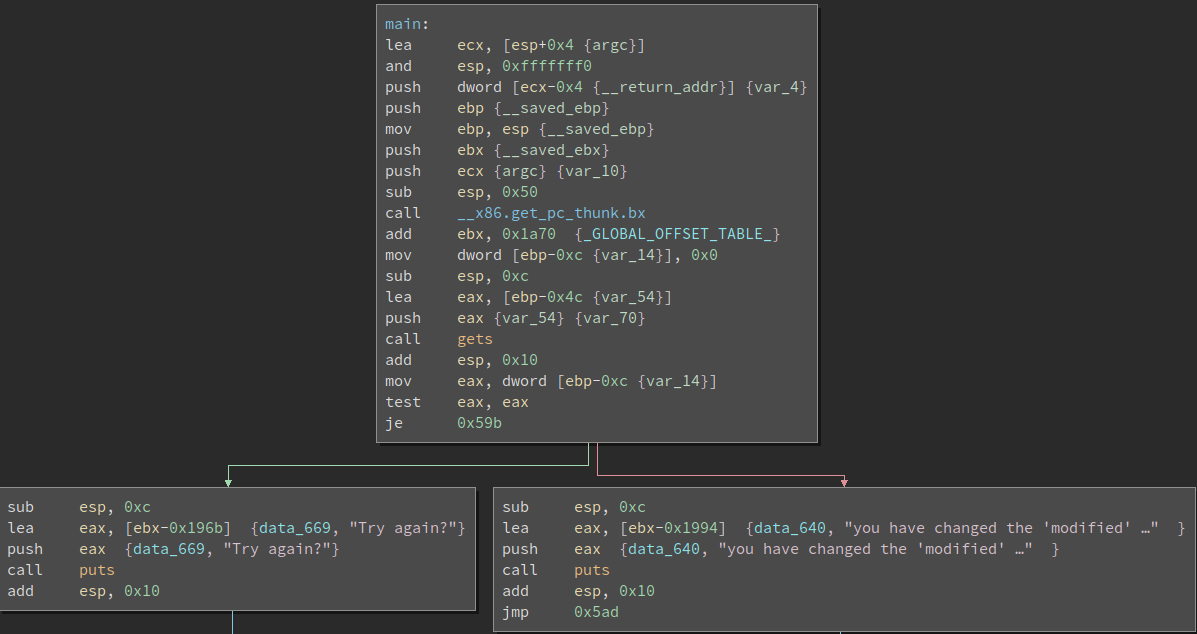
\includegraphics[scale=.4]{photos/p5pic1}
\end{center}

My suspicions were confirmed true by looking at the binary, it seems the gets reads in too much data and overwrites some data,
although I am not exactly certain how many characters I need it doesn't really matter because we are able to exploit and get
the data we needed. 

%\newpage

%%%%%%%%%%%%%%%%%%%%%%%%%%%%%%%%%%%%%%%%%%%%%%%%%%%%%%%%%%%%%%%%%%%%%%%%%%%%%%%%%%
%                                                                                %
%                                   Problem 6                                    %
%                                                                                %
%%%%%%%%%%%%%%%%%%%%%%%%%%%%%%%%%%%%%%%%%%%%%%%%%%%%%%%%%%%%%%%%%%%%%%%%%%%%%%%%%%
\section{Problem 6}
\tab Analyze the vulnerable binary named “p6” and solve. Write up your solution

\textbf{\\Solution:\\}

\tab My initial instinct was to think this was an integer overflow. I thought it was an integer overflow
because when the program is run it asks ``\texttt{p6: please specify an argument}". I suspected, similarly to 
Problem 1 that this requires some file, and reading a larger amount of data than available will cause an integer
overflow. Let me try this out with an empty .txt file. When I passed an empty .txt file, running the command:
\texttt{./p6 stuff.txt}, and it read out ``\texttt{Try again, you got 0x00000000}". Okay, so maybe I am not supposed
get some sort of specific read, let me try to put in an extremely large string as the argument instead of the .txt. 
I put in about 50 of the letter `f' and got a different result, ``\texttt{Try again, you got 0x66666666}". This instead
seems to be a buffer overflow issue instead of an integer overflow. If I want to get any further I am going to need to 
observe the binaries. 

From here, I decide to open up Binary Ninja, and look for where the fail text, and hopefully correct text is. I notice
This in the binaries:

\begin{center}
	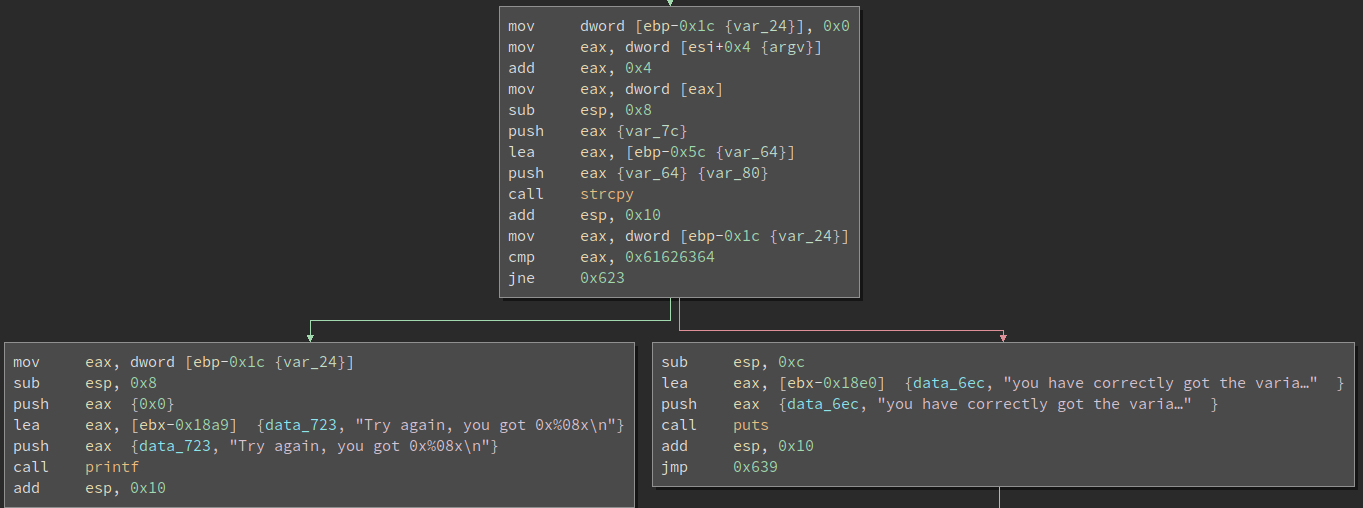
\includegraphics[scale=.45]{photos/p6pic1.png}
\end{center}

I see from here that the value I am looking for is \texttt{0x61626364}. Considering \texttt{f} correlates to values 
\texttt{66}, I can assume if we work backwards we will need to place the characters \texttt{dcba} at the right place. 
The problem is now the where, at what point do I place this \texttt{dcba}. I review the binaries some more to see exactly
at what point I see it. Looking through, it seems that, after counting, it is exactly 64 characters before it starts to
overflow into the integer. When we input 64 random chars and put in \texttt{dcba} there is a response of:
``\texttt{You have correctly got the variable to the right value}". 


%\newpage

%%%%%%%%%%%%%%%%%%%%%%%%%%%%%%%%%%%%%%%%%%%%%%%%%%%%%%%%%%%%%%%%%%%%%%%%%%%%%%%%%%
%                                                                                %
%                                   Problem 7                                    %
%                                                                                %
%%%%%%%%%%%%%%%%%%%%%%%%%%%%%%%%%%%%%%%%%%%%%%%%%%%%%%%%%%%%%%%%%%%%%%%%%%%%%%%%%%
\section{Problem 7}
\tab Analyze the vulnerable binary named “p7” and solve. Write up your solution

\textbf{\\Solution:}

This problem seems similar to the last problem. Essentially, I have to set an environment variable named \texttt{GREENIE}. When doing this, and setting it to a random assortment of characters it tells you that your memory fails, and spits out a hex value. Very confusingly, I decided to open up what was going on in Ghidra. I found something like this:
\begin{center}
	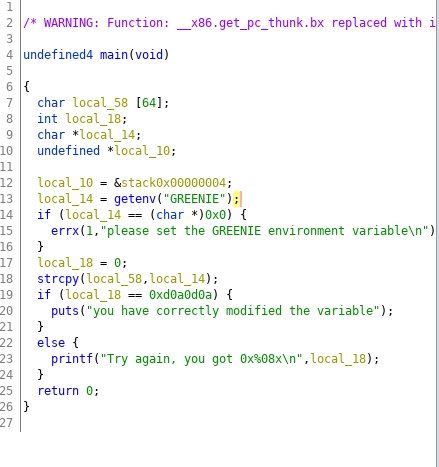
\includegraphics[scale=.7]{Photos/p7pic1.png}
\end{center}

What I see here is that there is a clear buffer overflow from \texttt{local\_58} into \texttt{local\_18}. What we have to do is put the value of \texttt{0xd0a0d0a} inside the environment after an initial placement of 64 characters. This is quite easy to do. We have to set the environemnt to be this character set, and we can get the message that we correctly modified the variable. 


\end{document}
